\documentclass[11pt,class=report,crop=false]{standalone}
\usepackage[screen]{../python}

\begin{document}


%====================================================================
\chapitre{Fichiers}
%====================================================================

\objectifs{Tu vas apprendre à lire et à écrire des données dans des fichiers.}

\begin{cours}[\'Ecrire dans un fichier]

\index{fichier}

\'Ecrire dans un fichier est presque aussi facile que d'afficher une phrase à l'écran.
Voici à gauche un programme qui écrit deux lignes dans un fichier appelé \ci{mon_fichier.txt} ; à droite le fichier résultant qui s'affiche dans un éditeur de texte.
\begin{center}
\begin{minipage}{0.5\textwidth}
\begin{lstlisting}
fic = open("mon_fichier.txt","w")

fic.write("Bonjour le monde\n")

ligne = "Coucou\n"
fic.write(ligne)

fic.close()
\end{lstlisting}
\end{minipage}
\begin{minipage}{0.3\textwidth}
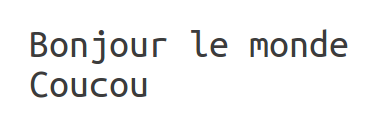
\includegraphics[scale=0.5]{ecran-fichiers-cours-1}
\end{minipage}
\end{center}


\textbf{Explications.}
\begin{itemize}
  \item La commande \ci{open}\index{open@\ci{open}} permet d'ouvrir un fichier. Le premier argument est le nom du fichier. Le second argument est ici \ci{"w"} pour dire que l'on veut écrire dans le fichier (\emph{write} en anglais).
  
  \item On ne travaille pas avec le nom du fichier, mais avec la valeur renvoyée par la fonction \ci{open}. Ici nous avons nommé \ci{fic} ce fichier-objet. C'est avec cette variable \ci{fic} que l'on travaille désormais.
  
  \item On écrit maintenant dans le fichier presque comme on afficherait une phrase à l'écran. L'instruction est \ci{fic.write()}\index{write@\ci{write}} où l'argument est une chaîne de caractères.
  
  \item Pour passer à la ligne, il faut ajouter le caractère de fin de ligne \ci{"\\n"}.
  
  \item Il est important de fermer son fichier quand on a fini d'écrire. La commande est \ci{fic.close()}.\index{close@\ci{close}} 
   
  \item Les données à écrire sont des chaînes, donc pour écrire un nombre, il faut d'abord le transformer par \ci{str(nombre)}.\index{str@\ci{str}}
\end{itemize}
  
  
\end{cours}


\begin{cours}[Lire un fichier]

C'est tout aussi facile de lire un fichier.
Voici comment faire (à gauche) et l'affichage par \Python{} à l'écran (à droite).
\begin{center}
\begin{minipage}{0.5\textwidth}
\begin{lstlisting}
fic = open("mon_fichier.txt","r")

for ligne in fic:
    print(ligne)

fic.close()
\end{lstlisting}
\end{minipage}
\begin{minipage}{0.3\textwidth}
\begin{lstlisting}
Bonjour le monde

Coucou
\end{lstlisting}
\end{minipage}
\end{center}

\textbf{Explications.}
\begin{itemize}
  \item La commande \ci{open} est cette fois appelée avec l'argument \ci{"r"} (pour \emph{read}), elle ouvre le fichier en lecture.
  
  \item On travaille de nouveau avec un fichier-objet nommé ici \ci{fic}.
  
  \item Une boucle parcourt tout le fichier ligne par ligne. Ici on demande juste l'affichage de chaque ligne.
  
  \item On ferme le fichier avec \ci{fic.close()}.  
  
  \item Les données lues sont des chaînes, donc pour obtenir un nombre, il faut d'abord le transformer par \ci{int(chaine)}\index{int@\ci{int}} (pour un entier) ou  
  \ci{float(chaine)}\index{chaine@chaîne} (pour un nombre à virgule).

\end{itemize}
  
\end{cours}



%%%%%%%%%%%%%%%%%%%%%%%%%%%%%%%%%%%%%%%%%%%%%%%%%%%%%%%%%%%%%%%%
% Activité 1
%%%%%%%%%%%%%%%%%%%%%%%%%%%%%%%%%%%%%%%%%%%%%%%%%%%%%%%%%%%%%%%%

\begin{activite}[Lire et écrire un fichier]

\objectifs{Objectifs : écrire un fichier de notes, puis le lire pour calculer les moyennes.}

\begin{enumerate}
  \item Génère au hasard un fichier de notes, nommé \ci{notes.txt}, qui est composé de lignes ayant la structure :\\
  \centerline{\ci{Prenom Nom note1 note2 note3}} 
  
  Par exemple :
\begin{center}
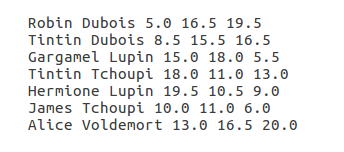
\includegraphics[scale=0.7]{ecran-fichiers-1a}
\end{center} 

  \emph{Indications.}
  \begin{itemize}
    	\item Construis un liste de prénoms \ci{liste_prenoms = ["Tintin","Harry","Alice",...]}. Puis choisis un prénom au hasard par la commande
    	\ci{prenom = choice(liste_prenoms)}.\index{choice@\ci{choice}} (il faut importer le module \ci{random}).
    	
    	\item Même chose pour les noms ! 
    	
    	\item Pour une note, tu peux choisir un nombre au hasard avec la commande  \ci{randint(a,b)}. 
    	
    	\item \textbf{Attention !} N'oublie pas de convertir les nombres en une chaîne de caractères pour l'écrire dans le fichier : \ci{str(note)}.
    	
   \end{itemize}
    
  
  \item Lis le fichier \ci{notes.txt} que tu as produit. Calcule la moyenne de chaque personne et écrit le résultat dans un fichier \ci{moyennes.txt} où chaque ligne est de la forme :\\
  \centerline{\ci{Prenom Nom moyenne}} 
  
    Par exemple :
\begin{center}
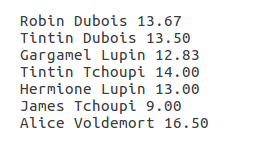
\includegraphics[scale=0.7]{ecran-fichiers-1b}
\end{center}  

  \emph{Indications.}
  \begin{itemize}
    	\item Pour chaque ligne lue du fichier \ci{notes.txt}, tu récupères les données dans  une liste par la commande \ci{ligne.split()}.
    	
    	\item \textbf{Attention !} Les données lues sont des chaînes de caractères. Tu peux convertir une chaîne \ci{"12.5"} en le nombre \ci{12.5} par la commande \ci{float(chaine)}.
    	
    	\item Pour convertir une nombre en une chaîne avec seulement deux décimales après la virgule, tu peux utiliser la commande \ci{'\{0:.2f\}'.format(moyenne)}.
    	
    	\item N'oublie pas de fermer tous tes fichiers.
    	
   \end{itemize}
    
\end{enumerate}   
     
\end{activite}


%%%%%%%%%%%%%%%%%%%%%%%%%%%%%%%%%%%%%%%%%%%%%%%%%%%%%%%%%%%%%%%%
%%%%%%%%%%%%%%%%%%%%%%%%%%%%%%%%%%%%%%%%%%%%%%%%%%%%%%%%%%%%%%%%

\begin{cours}[Fichiers au format \emph{csv}]
Le format \emph{csv}\index{csv@\emph{csv}} (pour  \emph{comma-separated values}) est un format très simple de fichier texte contenant des données.
Chaque ligne du fichier contient des données (des nombres ou du texte). Sur une même ligne les données sont séparées par une virgule (d'où le nom du format, même si d'autres séparateurs sont possibles).

\textbf{Exemple.} Voici un fichier qui contient les noms, prénoms, années de naissances, la taille ainsi que le nombre de prix Nobel reçus :
 \begin{center}
\begin{minipage}{0.4\textwidth}
\begin{lstlisting}
CURIE,Marie,1867,1.55,2
EINSTEIN,Albert,1879,1.75,1
NOBEL,Alfed,1833,1.70,0
\end{lstlisting}
\end{minipage}
\end{center}

\end{cours}


%%%%%%%%%%%%%%%%%%%%%%%%%%%%%%%%%%%%%%%%%%%%%%%%%%%%%%%%%%%%%%%%
% Activité 2
%%%%%%%%%%%%%%%%%%%%%%%%%%%%%%%%%%%%%%%%%%%%%%%%%%%%%%%%%%%%%%%%


\begin{activite}[]

\objectifs{Objectifs : écrire un fichier de données au format \emph{csv}, puis le lire pour un affichage graphique.}

\begin{enumerate}
  \item Génère  un fichier \ci{ventes.csv} des chiffres de ventes (tirés au hasard) d'une enseigne de sport.
  
Voici un exemple :
\begin{center}
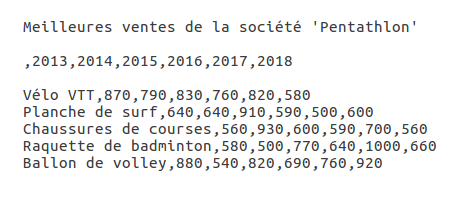
\includegraphics[scale=0.6]{ecran-fichiers-2a}
\end{center} 

\begin{itemize}
  \item Les données débutent à partir de la cinquième ligne.
  \item Le fichier produit respecte le format \emph{csv} et doit pouvoir être lu par
   \emph{LibreOffice Calc} par exemple.
\end{itemize}

\begin{center}
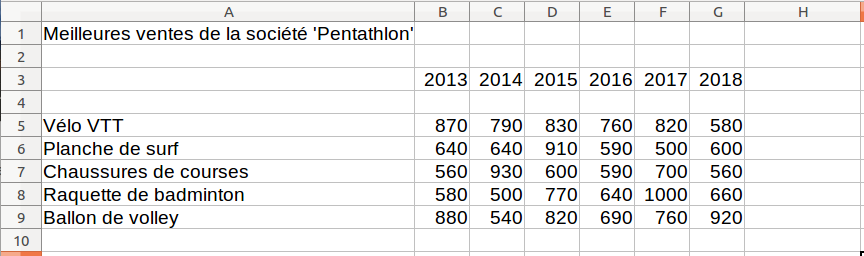
\includegraphics[scale=0.4]{ecran-fichiers-2b}
\end{center} 

  \item Lit le fichier \ci{ventes.csv} pour afficher les courbes de ventes.
  \begin{center}
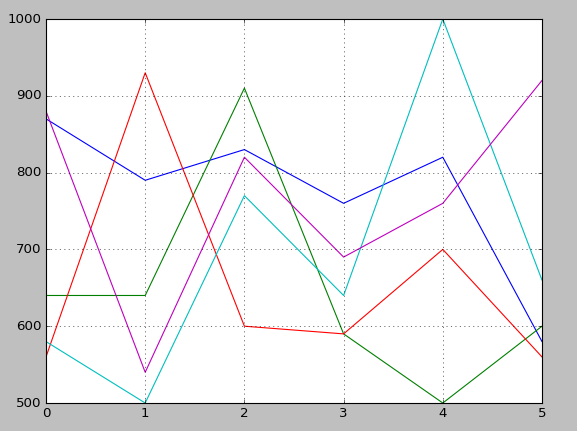
\includegraphics[scale=0.5]{ecran-fichiers-2c}
\end{center}  

  \emph{Indications.} 
  \begin{itemize}
    	\item Le package \ci{matplotlib} permet d'afficher facilement des graphiques, il s'appelle souvent selon l'instruction :\\
   \centerline{\ci{import matplotlib.pyplot as plt}}  
   
   \item Voici comment visualiser deux listes de données \ci{liste1} et \ci{liste2} :
\begin{center}
\begin{minipage}{0.4\textwidth}
\begin{lstlisting}
plt.plot(liste1)
plt.plot(liste2)
plt.grid()
plt.show()
\end{lstlisting}
\end{minipage}
\end{center}


   \end{itemize}
\end{enumerate}   
     
\end{activite}

%%%%%%%%%%%%%%%%%%%%%%%%%%%%%%%%%%%%%%%%%%%%%%%%%%%%%%%%%%%%%%%%
%%%%%%%%%%%%%%%%%%%%%%%%%%%%%%%%%%%%%%%%%%%%%%%%%%%%%%%%%%%%%%%%


\begin{cours}[Images \emph{bitmap}]

\index{pbm@\emph{pbm/pgm/ppm}}
\index{image}

Il existe un format simple de fichier, appelé format \emph{bitmap}, qui décrit pixel par pixel une image. Ce format se décline en trois variantes 
selon que l'image est en noir et blanc, en niveaux de gris ou bien en couleur.

\medskip

\textbf{Image noir et blanc, le format \og{}pbm\fg{}.}

L'image est décrite par des $0$ et des $1$.

Voici un exemple : le fichier \ci{image_nb.pbm} à gauche (lu comme un fichier texte)  et à droite sa visualisation (à l'aide d'un lecteur d'images, ici très agrandi).
\begin{center}
\begin{minipage}{0.3\textwidth}
\begin{lstlisting}
P1
4 5
1 1 1 1
1 0 0 0
1 1 1 0
1 0 0 0
1 1 1 1
\end{lstlisting}
\end{minipage}
\begin{minipage}{0.3\textwidth}

\includegraphics[scale=0.2]{ecran-cours-image_nb}
\end{minipage}
\end{center}

Voici la description du format :
\begin{itemize}
  \item Première ligne : l'identifiant \ci{P1}.
  \item Deuxième ligne : le nombre de colonnes puis le nombre de lignes (ici 4 colonnes et 5 lignes).
  \item Puis la couleur de chaque pixel ligne par ligne : \ci{1} pour un pixel noir, \ci{0} pour un pixel blanc. Attention : c'est contraire à la convention habituelle !
\end{itemize}  
  
\medskip

\textbf{Image en niveaux de gris, le format \og{}pgm\fg{}.}

L'image est décrite par différentes valeurs pour différents niveaux de gris.
Voici un exemple : le fichier \ci{image_gris.pbm} à gauche et à droite sa visualisation.
\begin{center}
\begin{minipage}{0.3\textwidth}
\begin{lstlisting}
P2
4 5
255
  0   0   0   0
192 192 192 192
192 255 128 128
192 255  64  64
192   0   0   0
\end{lstlisting}
\end{minipage}
\begin{minipage}{0.3\textwidth}

\includegraphics[scale=0.2]{ecran-cours-image_gris}
\end{minipage}
\end{center}

Voici la description du format :
\begin{itemize}
  \item Première ligne : l'identifiant est cette fois \ci{P2}.
  \item Deuxième ligne : le nombre de colonnes puis le nombre de lignes.
  \item Troisième ligne : la valeur maximale du niveau de gris (ici $255$).
  \item Puis le niveau de gris de chaque pixel ligne par ligne : cette fois \ci{0} pour un pixel noir, la valeur maximale pour un pixel blanc et les valeurs intermédiaires donnent des gris. 
\end{itemize}  

\medskip

\textbf{Image en couleurs, le format \og{}ppm\fg{}.}


L'image est décrite par trois valeurs par pixel : une pour le rouge, une pour le vert, une pour le bleu.

Voici un exemple : le fichier \ci{image_coul.ppm} à gauche et à droite sa visualisation.
\begin{center}
\begin{minipage}{0.6\textwidth}
\begin{lstlisting}
P3
3 2
255
255   0   0     0 255 0     0   0 255
  0 128 255   255 128 0   128 255   0
\end{lstlisting}
\end{minipage}
\begin{minipage}{0.3\textwidth}
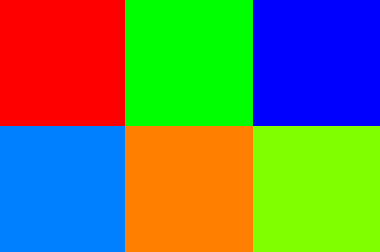
\includegraphics[scale=0.2]{ecran-cours-image_coul}
\end{minipage}
\end{center}

Voici la description du format :
\begin{itemize}
  \item Première ligne : l'identifiant est maintenant \ci{P3}.
  \item Deuxième ligne : le nombre de colonnes puis le nombre de lignes.
  \item Troisième ligne : la valeur maximale des niveaux de couleur (ici $255$).
  \item Puis chaque pixel est décrit par $3$ nombres : le niveau de rouge, celui de vert puis celui de bleu (système RVB, \emph{RGB} en anglais)\index{rvb@rvb/\emph{rgb}}. Par exemple le premier pixel est codé par $(255,0,0)$ c'est donc un pixel rouge.
\end{itemize} 


\end{cours}


%%%%%%%%%%%%%%%%%%%%%%%%%%%%%%%%%%%%%%%%%%%%%%%%%%%%%%%%%%%%%%%%
% Activité 3
%%%%%%%%%%%%%%%%%%%%%%%%%%%%%%%%%%%%%%%%%%%%%%%%%%%%%%%%%%%%%%%%

\begin{activite}[Images \emph{bitmap}]

\objectifs{Objectifs : définir tes propres images pixel par pixel.}


\begin{enumerate}
  \item Génère un fichier \ci{image_nb.pbm} qui représente une image en noir et blanc (par exemple de taille $300 \times 200$) selon le motif suivant :
\begin{center}

\includegraphics[scale=0.5]{ecran-image_nb}
\end{center}   

\emph{Indications.} Si $i$ désigne le numéro de ligne et $j$ le numéro de colonne (en partant du haut à gauche), alors le pixel en position $(i,j)$ est blanc si $i+j$ est compris entre $0$ et $9$, ou compris entre $20$ et $29$, ou entre $40$ et $49$,\ldots{} Ce qui s'obtient par la formule :\\
\centerline{\ci{coul = (i+j)//10 \% 2}}
qui renvoie $0$ ou $1$ comme désiré.

  \item  Génère un fichier \ci{image_gris.pgm} qui représente une image en niveaux de gris (par exemple de taille $200 \times 200$ avec $256$ niveaux de gris) selon le motif suivant :
\begin{center}
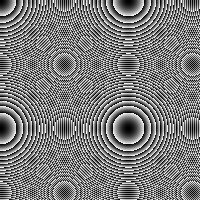
\includegraphics[scale=0.7]{ecran-image_gris}
\end{center}   

\emph{Indications.} Cette fois la formule est :\\
\centerline{\ci{coul = (i**2 + j**2) \% 256}}
qui renvoie un entier entre $0$ et $255$.

   \item Génère un fichier \ci{image_coul.ppm} qui représente une image en couleurs (par exemple de taille $200 \times 200$ avec $256$ niveaux de rouge, vert et bleu) selon le motif suivant :
\begin{center}
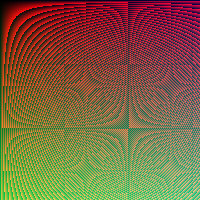
\includegraphics[scale=0.7]{ecran-image_coul}
\end{center}   

\emph{Indications.} Cette fois la formule est :\\
\centerline{\ci{R = (i*j) \% 256}}
\centerline{\ci{V = i \% 256}}
\centerline{\ci{B = (i + j)//3 \% 256}}
qui donne les niveaux de rouge, vert et bleu du pixel $(i,j)$.

\item Écris une fonction \ci{inverser_couleurs_nb(fichier)} qui lit un fichier image noir et blanc \ci{.pbm} et crée un nouveau fichier dans lequel les pixels blancs sont devenus noirs et inversement. 

Exemple : à gauche l'image de départ, à droite l'image d'arrivée.
\begin{center}

\includegraphics[scale=0.3]{ecran-simple_nb}\qquad\qquad

\includegraphics[scale=0.3]{ecran-simple_nb_inverse}
\end{center} 

\item Écris une fonction \ci{couleurs_vers_gris(fichier)} qui lit un fichier image couleur au format \ci{.ppm} et crée un nouveau fichier au format \ci{.pgm} dans lequel les pixels couleurs sont transformés en niveaux de gris. 

Tu peux utiliser la formule :\index{rvb@rvb/\emph{rgb}}
$$G = 0,21 \times R \  + \  0,72 \times V \  + \  0,07 \times B$$
où
\begin{itemize}
  \item $R,V,B$ sont les niveaux de rouge, vert et bleu du pixel coloré,
  \item $G$ est le niveau de gris du pixel transformé.
\end{itemize}

Exemple : à gauche l'image de départ en couleur, à droite l'image d'arrivée en niveau de gris.
\begin{center}
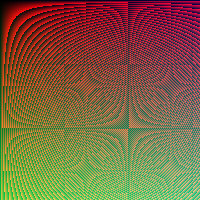
\includegraphics[scale=0.5]{ecran-image_coul}\qquad\qquad
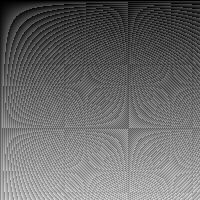
\includegraphics[scale=0.5]{ecran-image_coul_gris}
\end{center} 


\end{enumerate}   
     
\end{activite}


%%%%%%%%%%%%%%%%%%%%%%%%%%%%%%%%%%%%%%%%%%%%%%%%%%%%%%%%%%%%%%%%
% Activité 4
%%%%%%%%%%%%%%%%%%%%%%%%%%%%%%%%%%%%%%%%%%%%%%%%%%%%%%%%%%%%%%%%


\begin{activite}[Distance entre deux villes]

\objectifs{Objectifs : lire les coordonnées des villes et écrire les distances entre elles.}
\index{distance}

\begin{enumerate}
  \item \textbf{Distance dans le plan.} 
  
  Écris un programme qui lit un fichier contenant les coordonnées $(x,y)$ de villes, puis qui calcule et écrit dans un autre fichier les distances (dans le plan) entre deux villes.
  
  La formule pour la distance entre deux points $(x_1,y_1)$ et $(x_2,y_2)$ du plan est :
  $$d = \sqrt{(x_2-x_1)^2 + (y_2-y_1)^2}.$$
  
  
\textbf{Exemple.} Voici un exemple de fichier en entrée :
\begin{center}
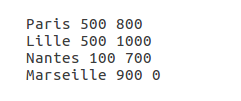
\includegraphics[scale=0.7]{ecran-fichiers-4a}
\end{center}   

Et voici le fichier de sortie produit par le programme :
\begin{center}
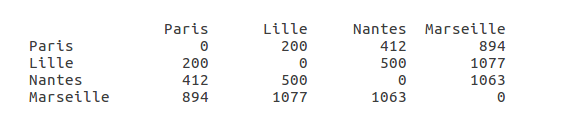
\includegraphics[scale=0.7]{ecran-fichiers-4b} 
\end{center}   
On lit sur ce fichier que la distance entre Lille et Marseille est de $1077$ kilomètres.


Ci-dessous la carte de France qui a fourni des données (très approximatives) pour le fichier d'entrée. L'origine est en bas à gauche, chaque côté d'un carré représente $100$ km. Par exemple, dans ce repère, Paris a pour coordonnées $(500,800)$.
 
 \myfigure{0.6}{
  \tikzinput{fig-france}
} 


  \item \textbf{Distance sur la sphère.} 
  
Sur la Terre, la distance entre deux villes correspond à un trajet suivant un \emph{grand cercle} à la surface de la sphère et pas selon une ligne droite. C'est la distance que parcourt un avion pour relier deux villes.

 Écris un programme qui lit les latitudes et longitudes des villes, puis qui calcule et écrit dans un autre fichier les distances (à la surface de la Terre) entre deux villes. 
  
\textbf{Exemple.} Voici un exemple de fichier en entrée :
\begin{center}
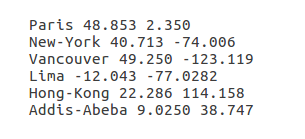
\includegraphics[scale=0.7]{ecran-fichiers-4c}
\end{center}   

Et voici le fichier de sortie produit par le programme :
\begin{center}
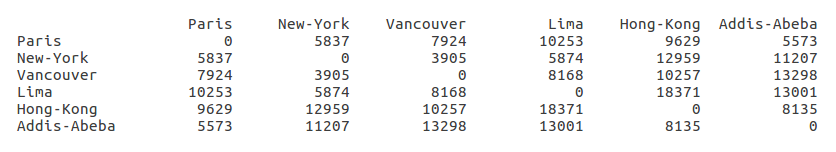
\includegraphics[scale=0.55]{ecran-fichiers-4d} 
\end{center}  
    
    
\textbf{Mise en \oe uvre et explications.}

\begin{itemize}
	\item Le fichier d'entrée contient la latitude (notée $\varphi$) et la longitude (notée $\lambda$) en degrés de chaque ville. Par exemple Paris a pour latitude $\varphi = 48.853$ degrés et pour longitude $\lambda = 2.350$ degrés.
	
	\item Pour les formules, il faudra utiliser les angles en radians. La formule de conversion de degrés vers radians est :\index{angle}\index{degres@degrés}\index{radians}
	$$\text{angle en radians} = \frac{2\pi}{360} \times \text{angle en degrés}$$
		
	\item \textbf{Formule de la distance approchée.}
	
	Il existe une formule simple qui donne une bonne estimation pour la distance la plus courte entre deux points d'une sphère de rayon $R$.
    Poser d'abord :
    $$x =   (\lambda_2-\lambda_1)\cdot  \cos\left( \frac{\varphi_1+\varphi_2}{2} \right)
    \quad\text{ et }\quad 
    y = \varphi_2-\varphi_1$$
	La distance approchée est alors 
	$$ \tilde d = R \sqrt{x^2 + y^2}$$	
	
	$(\varphi_1,\lambda_1)$ et $(\varphi_2,\lambda_2)$ sont les latitudes/longitudes de deux villes exprimées en radians.
	
	\item \textbf{Formule de la distance exacte.}
	
	Les plus courageux peuvent utiliser la formule exacte pour calculer la distance.
	Poser d'abord : 
	$$a = \left(\sin\left(\frac{\varphi_1+\varphi_2}{2}\right)\right)^2 + \cos(\varphi_1)\cdot \cos(\varphi_2) \cdot \left(\sin\left( \frac{\lambda_2-\lambda_1}{2} \right)\right)^2$$
    La distance exacte est alors :
    $$d = 2 \cdot R \cdot \text{atan2}\left(\sqrt{a},\sqrt{1-a}\right)$$
    où $\text{atan2}(y,x)$ est la fonction \og{}arctangente\fg{} qui s'obtient par la commande \ci{atan2(y,x)} du module \ci{math}.	
	
	\item Pour le rayon de la Terre on prendra $R = 6371$ km.

\end{itemize}
  
\end{enumerate}   
     
\end{activite}


\end{document}
